\chapter{Progressioni armoniche per l'armonizzazione del basso}
\label{chap:progressioni_armoniche}

Dopo aver studiato le funzioni armoniche, le cadenze e la Regola dell'Ottava, siamo pronti ad affrontare l'\textbf{armonizzazione di un basso dato}. Questo capitolo tratta le \textbf{progressioni armoniche}, successioni di accordi che si ripetono trasposte e servono ad armonizzare passaggi scalari, sequenze modulanti e movimenti melodici complessi.

\section{Che cos'è una progressione armonica}
\label{sec:definizione_progressione}

\begin{definizione}[Progressione armonica]
	\label{def:progressione_armonica}
	Una \textbf{progressione armonica} (o \textbf{sequenza armonica}) è una successione di accordi che viene ripetuta trasportata su diversi gradi della scala. Questa ripetizione crea un movimento armonico coerente e prevedibile che può essere utilizzato per costruire frasi musicali più lunghe o per effettuare modulazioni.
	
	Elementi caratteristici:
	\begin{itemize}
		\item \textbf{Schema di base (modello):} Una breve successione di accordi (tipicamente 2-4 accordi)
		\item \textbf{Trasposizione:} Il modello viene ripetuto su gradi diversi della scala
		\item \textbf{Direzione:} La progressione può muoversi verso l'acuto (ascendente) o verso il grave (discendente)
		\item \textbf{Numero di ripetizioni:} Tipicamente 2-4 volte, raramente di più per evitare monotonia
	\end{itemize}
\end{definizione}

Le progressioni armoniche sono particolarmente utili nell'armonizzazione del basso per diversi motivi:

\begin{itemize}
	\item Forniscono una soluzione sistematica per passaggi scalari lunghi
	\item Creano movimento e dinamismo armonico
	\item Facilitano la modulazione verso tonalità vicine
	\item Rendono il discorso musicale coerente e memorabile
\end{itemize}

\begin{fisica}[Perché le progressioni funzionano?]
	Dal punto di vista percettivo, le progressioni sfruttano il \textbf{riconoscimento di pattern}. 
	
	Il cervello identifica con facilità gli schemi ricorrenti. Quando ascoltiamo una progressione, dopo la prima o seconda ripetizione del modello, il nostro sistema cognitivo:
	\begin{enumerate}
		\item \textbf{Anticipa} il movimento successivo
		\item \textbf{Categorizza} il materiale come "coerente"
		\item \textbf{Elabora} più facilmente la struttura complessiva
	\end{enumerate}
	
	Per questo le progressioni risultano naturali all'ascolto: creano varietà armonica in un modo che il cervello segue agevolmente.
\end{fisica}

\section{Progressioni fondamentali}
\label{sec:progressioni_fondamentali}

Esistono diverse famiglie di progressioni, classificabili in base alla direzione del movimento armonico. Le più comuni sono le progressioni per \textbf{quinte discendenti} (o quarte ascendenti) e le progressioni per \textbf{terze} (ascendenti o discendenti).

\subsection{Progressione per quinte discendenti}
\label{subsec:progressione_quinte}

La progressione per quinte discendenti è una delle più naturali nel sistema tonale, perché replica il movimento cadenzale V-I su ogni grado della scala.

\begin{regola}[Progressione per quinte discendenti]
	\label{reg:progressione_quinte_disc}
	Nella \textbf{progressione per quinte discendenti}, ogni accordo viene seguito da un altro la cui fondamentale è una quinta sotto (o una quarta sopra). La successione tipica è:
	
	\textbf{Nel modo maggiore:}
	I - IV - VII - III - VI - II - V - I
	
	\textbf{Nel modo minore:}
	i - iv - VII - III - VI - ii° - V - i
	
	Caratteristiche:
	\begin{itemize}
		\item Il movimento del basso procede per \textbf{quarte ascendenti} (equivalente intervallare della quinta discendente)
		\item Gli accordi alternano generalmente stati fondamentali e primi rivolti per mantenere il movimento del basso fluido
		\item La sensazione armonica è di continua "risoluzione" e direzione verso la tonica
	\end{itemize}
\end{regola}

\begin{esempio}[Progressione per quinte discendenti in Do Maggiore]
	\label{ex:progressione_quinte_disc}
	Progressione completa con alternanza di stati fondamentali e rivolti.
	\musica{es_cap17_01}
	
	Notare come l'alternanza tra stato fondamentale (5) e primo rivolto (6) mantiene il basso in movimento per grado congiunto o salti piccoli, evitando salti eccessivi.
\end{esempio}

\begin{matematica}[Il cerchio delle quinte e la progressione]
	La progressione per quinte discendenti non è altro che una "passeggiata" lungo il \textbf{cerchio delle quinte}. Questo cerchio può essere rappresentato come un grafo ciclico dove ogni nodo rappresenta una tonalità e gli archi connettono tonalità adiacenti per quinte.
	
	Se rappresentiamo le 7 note diatoniche di Do Maggiore sul cerchio delle quinte, otteniamo:
	
	\begin{center}
	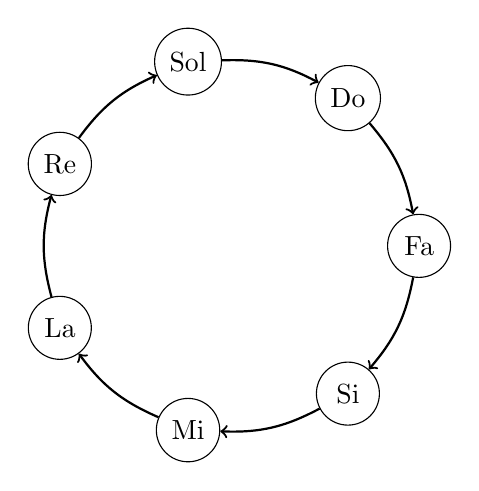
\begin{tikzpicture}[scale=1.2]
		\foreach \note/\angle in {Fa/0, Do/51.43, Sol/102.86, Re/154.29, La/205.71, Mi/257.14, Si/308.57} {
			\node[circle, draw, minimum size=0.8cm] (\note) at (\angle:2cm) {\note};
		}
		\draw[->, thick] (Do) to[bend left=15] (Fa);
		\draw[->, thick] (Fa) to[bend left=15] (Si);
		\draw[->, thick] (Si) to[bend left=15] (Mi);
		\draw[->, thick] (Mi) to[bend left=15] (La);
		\draw[->, thick] (La) to[bend left=15] (Re);
		\draw[->, thick] (Re) to[bend left=15] (Sol);
		\draw[->, thick] (Sol) to[bend left=15] (Do);
	\end{tikzpicture}
	\end{center}
	
	La progressione per quinte discendenti percorre questo cerchio in senso antiorario. Dal punto di vista della teoria dei grafi, questo è un \textbf{cammino hamiltoniano} sul sottografo ciclico delle note diatoniche.
	
	In temperamento equabile, dopo 12 quinte giuste si torna alla nota di partenza (a meno di una piccola discrepanza chiamata \textit{comma pitagorico}), ma nel sistema diatonico, dopo 7 passi si ritorna alla tonica originale.
\end{matematica}

\subsection{Progressione per terze discendenti}
\label{subsec:progressione_terze_disc}

La progressione per terze discendenti crea un movimento armonico più morbido rispetto a quella per quinte.

\begin{regola}[Progressione per terze discendenti]
	\label{reg:progressione_terze_disc}
	Nella \textbf{progressione per terze discendenti}, ogni accordo scende di terza (maggiore o minore) rispetto al precedente. Una forma comune è:
	
	\textbf{Nel modo maggiore:}
	I - VI - IV - II - VII - V - I
	
	Caratteristiche:
	\begin{itemize}
		\item Il movimento è più graduale e "dolce" rispetto alla progressione per quinte
		\item Spesso utilizzata in passaggi espressivi o melanconici
		\item Il basso può muoversi per terze o, più frequentemente, per grado congiunto usando rivolti appropriati
	\end{itemize}
\end{regola}

\begin{esempio}[Progressione per terze discendenti in Do Maggiore]
	\label{ex:progressione_terze_disc}
	Sequenza che scende per terze con movimento del basso per grado congiunto.
	\musica{es_cap17_02}
	Questa progressione scende attraverso la scala, creando una sensazione di dolce malinconia.
\end{esempio}

\section{Applicazione pratica: armonizzare un basso dato}
\label{sec:applicazione_basso_dato}

Ecco un metodo sistematico per riconoscere quando e come applicare le progressioni.

\begin{regola}[Strategia per l'armonizzazione del basso]
	\label{reg:strategia-armonizzazione}
	Quando ci troviamo di fronte a un basso da armonizzare, seguire questi passi:
	
	\begin{enumerate}
		\item \textbf{Identificare la struttura:}
		\begin{itemize}
			\item Cadenze (dove si trovano i punti di riposo?)
			\item Passaggi scalari (ascendenti o discendenti)
			\item Salti significativi (quarte, quinte, ottave)
		\end{itemize}
		
		\item \textbf{Scegliere la tecnica appropriata:}
		\begin{itemize}
			\item Per \textbf{movimenti scalari brevi} (2-4 note): applicare la Regola dell'Ottava
			\item Per \textbf{movimenti scalari lunghi} (5+ note): considerare progressioni
			\item Per \textbf{salti}: usare prevalentemente stati fondamentali
		\end{itemize}
		
		\item \textbf{Applicare le progressioni:}
		\begin{itemize}
			\item Identificare il pattern che il basso suggerisce (quinte, terze, seconde?)
			\item Applicare la progressione appropriata
			\item Verificare che la condotta delle voci sia corretta
		\end{itemize}
		
		\item \textbf{Raffinare:}
		\begin{itemize}
			\item Correggere parallelismi
			\item Migliorare il canto (linea del soprano)
			\item Aggiungere varietà ritmica se necessario
		\end{itemize}
	\end{enumerate}
\end{regola}

\begin{esempio}[Basso dato con progressione per quinte]
	\label{ex:basso_dato_progressione}
	
	\textbf{Basso da armonizzare:}
	\musica{es_cap17_03}
	
	\textbf{Analisi:}
	\begin{itemize}
		\item Battuta 1: salto Do-Fa (quarta) suggerisce I-IV
		\item Fa-Sol-Do': parte di una progressione per quinte (IV-VII-III o IV-V-I)
		\item Battuta 2: La-Re-Sol-Do continua la discesa per quinte
	\end{itemize}
	
	\textbf{Soluzione armonizzata:}
	\musica{es_cap17_04}
	
	La progressione per quinte (IV-V-III-VI-II-V-I) permette di creare un movimento armonico fluido e convincente.
\end{esempio}

\section{Progressioni con settime}
\label{sec:progressioni_settime}

Le settime nelle progressioni aumentano la tensione direzionale.

\begin{regola}[Progressioni di settime]
	\label{reg:progressioni_settime}
	Nelle progressioni, le settime possono essere impiegate in due modi:
	
	\begin{enumerate}
		\item \textbf{Settime alternate:} Solo alcuni accordi della progressione hanno la settima
		\item \textbf{Settime consecutive:} Ogni accordo della progressione è un accordo di settima
	\end{enumerate}
	
	Nel caso di settime consecutive, la condotta delle voci segue una regola precisa:
	\begin{itemize}
		\item La settima di ciascun accordo \textbf{scende di grado} nell'accordo successivo
		\item Questa nota diventa spesso la \textbf{terza} dell'accordo successivo
		\item Il pattern crea una "catena" di risoluzioni che lega gli accordi
	\end{itemize}
\end{regola}

\begin{esempio}[Progressione per quinte con settime consecutive]
	\label{ex:progressione_settime}
	Ogni accordo è una settima che risolve nel successivo.
	\musica{es_cap17_05}
	
	Notare come ogni settima (Fa nel \sigla{II}{7}{}, Fa nel \sigla{V}{7}{}, Si nel \sigla{I}{7}{}, Mi nel \sigla{IV}{7}{}) scende di grado per diventare la terza dell'accordo successivo.
\end{esempio}

\begin{errore}[Progressioni troppo lunghe]
	\label{err:progressioni_lunghe}
	Un errore comune è quello di applicare meccanicamente una progressione per troppe ripetizioni, creando monotonia. 
	
	\textbf{Problema:}
	\musica{es_cap17_06}
	
	Questa progressione per quinte discendenti si estende per tre battute complete, risultando meccanica e prevedibile.
	
	\textbf{Soluzione:}
	Interrompere la progressione dopo 2-3 cicli e introdurre varietà:
	\begin{itemize}
		\item Usare una cadenza per chiudere la frase
		\item Cambiare tipo di progressione
		\item Inserire un accordo di passaggio o nota pedale
	\end{itemize}
	
	In generale, raramente si dovrebbero superare le 3-4 ripetizioni consecutive dello stesso modello.
\end{errore}

\section{Progressioni modulanti}
\label{sec:progressioni_modulanti}

Le progressioni possono facilitare la modulazione verso tonalità vicine.

\begin{definizione}[Progressione modulante]
	\label{def:progressione_modulante}
	Una \textbf{progressione modulante} è una sequenza armonica che, attraverso le sue ripetizioni trasposte, conduce naturalmente da una tonalità a un'altra. La modulazione avviene spesso in modo graduale e quasi impercettibile, sfruttando la coerenza del pattern ripetitivo.
\end{definizione}

\begin{regola}[Modulazione attraverso progressioni]
	\label{reg:modulazione_progressioni}
	Per modulare usando una progressione:
	
	\begin{enumerate}
		\item Iniziare la progressione nella tonalità di partenza
		\item Continuare il pattern introducendo gradualmente alterazioni che appartengono alla nuova tonalità
		\item Confermare la nuova tonalità con una cadenza autentica
	\end{enumerate}
	
	Le progressioni per quinte discendenti sono particolarmente efficaci perché:
	\begin{itemize}
		\item Ogni "quinta" può potenzialmente diventare una dominante della tonalità successiva
		\item L'introduzione di alterazioni cromatiche (es. \# per creare sensibili) avviene naturalmente
		\item Il movimento è direzionale e porta organicamente verso la nuova tonica
	\end{itemize}
\end{regola}

\begin{esempio}[Progressione modulante: da Do Maggiore a Sol Maggiore]
	\label{ex:progressione_modulante}
	Una progressione per quinte che modula al tono della dominante.
	\musica{es_cap17_07}
	
	Il \Fadiesis  introdotto nel secondo accordo trasforma il VII° di Do in V di Sol, preparando la modulazione. La conferma avviene con la cadenza II-V-I in Sol Maggiore.
\end{esempio}

\section{Esercizi di armonizzazione}
\label{sec:esercizi_progressioni}

Per padroneggiare le progressioni, serve esercitarsi con bassi dati di complessità crescente.

\begin{esempio}[Esercizio 1: Basso con progressione per quinte]
	\label{ex:esercizio_1}
	
	\textbf{Basso da armonizzare:}
	\musica{es_cap17_08}
	
	\textbf{Suggerimenti:}
	\begin{itemize}
		\item Identificare la progressione per quinte: Sol-Do (I-IV), Do-Si (IV-III), Si-La (III-II), La-Re-Sol (II-V-I)
		\item Usare rivolti per mantenere il movimento fluido del basso
		\item Fare attenzione alla condotta della sensibile (\Fadiesis )
	\end{itemize}
\end{esempio}

\begin{esempio}[Esercizio 2: Basso con salita scalare]
	\label{ex:esercizio_2}
	
	\textbf{Basso da armonizzare:}
	\musica{es_cap17_09}
	
	\textbf{Suggerimenti:}
	\begin{itemize}
		\item Riconoscere la salita scalare Fa-Sol-La-\Sibemolle -Do
		\item Il \Mibemolle  introduce una breve colorazione cromatica
		\item Applicare l'alternanza 6-5 tipica della salita scalare
		\item Concludere con cadenza plagale o autentica
	\end{itemize}
\end{esempio}

\begin{esempio}[Esercizio 3: Basso misto (Regola dell'Ottava + Progressione)]
	\label{ex:esercizio_3}
	
	\textbf{Basso da armonizzare:}
	\musica{es_cap17_10}
	
	\textbf{Suggerimenti:}
	\begin{itemize}
		\item Battuta 1 (Re-Mi-Fa-Sol): applicare Regola dell'Ottava ascendente
		\item Battuta 2 (La-\Sibemolle -Do-La): breve progressione (IV-V-VI-IV) o cadenza d'inganno
		\item Combinare le due tecniche per creare un'armonizzazione coerente
	\end{itemize}
\end{esempio}

\section{Progressioni nella letteratura musicale}
\label{sec:progressioni_letteratura}

Le progressioni armoniche sono una delle tecniche compositive più usate nella storia della musica.

\begin{fisica}[La "fisica" delle progressioni: energia armonica]
	Possiamo pensare alle progressioni armoniche in termini di \textbf{energia potenziale armonica}. Ogni accordo in una tonalità possiede un certo livello di "tensione" rispetto alla tonica:
	
	\begin{itemize}
		\item \textbf{Tonica (I):} Energia minima (riposo)
		\item \textbf{Dominante (V):} Energia massima (tensione)
		\item \textbf{Altri gradi:} Livelli intermedi
	\end{itemize}
	
	Le progressioni possono essere viste come "percorsi" attraverso questo paesaggio energetico:
	
	\begin{enumerate}
		\item \textbf{Progressione per quinte discendenti}: Simile a una "cascata" energetica dove ogni accordo "cade" verso il successivo (come dominante locale)
		
		\item \textbf{Salita scalare}: come una "salita" graduale che accumula tensione fino a un punto di rilascio
		
		\item \textbf{Progressione per terze}: Movimento più "orizzontale", mantenendo livelli energetici simili
	\end{enumerate}
	
\end{fisica}

\section{Progressioni con salti di quinta e di quarta}
\label{sec:progressioni_salti_quinta}

Oltre alle progressioni scalari che abbiamo finora esaminato, esistono progressioni particolarmente efficaci che si basano su \textbf{salti di quinta} (o quarta, che è l'inversione intervallare della quinta) nel basso. Queste progressioni creano un movimento armonico diretto, adatto a passaggi virtuosistici o a stabilire con forza il centro tonale.

\subsection{Progressione di quinte con numera 5}
\label{subsec:progressione_quinte_5}

La progressione più semplice e diretta con salti di quinta prevede l'uso di \textbf{accordi allo stato fondamentale} (numerati tutti 5, o senza numerazione esplicita). Il basso si muove per salti di quinta discendente (o quarta ascendente), e ogni accordo è presentato nella sua forma più stabile.

\begin{regola}[Progressione per quinte discendenti (tutti 5)]
	\label{reg:progressione_5}
	Nella progressione per salti di quinta con accordi allo stato fondamentale:
	
	\begin{itemize}
		\item Il \textbf{basso} si muove per salti di quinta discendente (o quarta ascendente)
		\item Tutti gli accordi sono allo \textbf{stato fondamentale} (cifra 5 o non numerati)
		\item Schema tipico: I - IV - VII - III - VI - II - V - I
		\item La condotta delle voci richiede particolare attenzione per evitare quinte e ottave parallele
	\end{itemize}
	
	\textbf{Tecnica di condotta delle voci:}
	Nel collegamento tra due accordi allo stato fondamentale con basso che salta di quinta, una tecnica efficace è muovere le tre voci superiori in \textbf{moto contrario} rispetto al basso, oppure mantenere una o due note comuni quando possibile.
\end{regola}

\begin{esempio}[Progressione per quinte discendenti (tutti 5) in Sol Maggiore]
	\label{ex:progressione_5_sol}
	Una sequenza di accordi tutti allo stato fondamentale.
	\musica{es_cap17_11}
	
	In questo esempio, il basso salta per quinte discendenti (Sol-Do-Mi-La-Sol), creando una forte progressione cadenzale. Notare che per evitare problemi di condotta si può usare occasionalmente un rivolto (come il \sigla{VII}{6}{} nell'esempio).
\end{esempio}

\subsection{Progressione di quinte con numera 7 (catena di settime)}
\label{subsec:progressione_quinte_7}

Una variante più sofisticata della progressione per quinte prevede l'uso sistematico di \textbf{accordi di settima}, tutti allo stato fondamentale. Questa tecnica, chiamata anche \textbf{catena di settime}, crea un movimento armonico particolarmente fluido.

\begin{regola}[Progressione per quinte con accordi di settima (tutti 7)]
	\label{reg:progressione_7}
	Nella \textbf{catena di settime}:
	
	\begin{itemize}
		\item Ogni accordo è una \textbf{settima} allo stato fondamentale (numerato 7)
		\item Il basso si muove per salti di quinta discendente (o quarta ascendente)
		\item La settima di ogni accordo \textbf{deve essere preparata} (apparire come consonanza nell'accordo precedente)
		\item La settima \textbf{risolve scendendo di grado} nell'accordo successivo
		\item Questa tecnica crea un movimento quasi automatico delle voci
	\end{itemize}
	
	\textbf{Meccanismo della risoluzione:}
	La settima di un accordo diventa automaticamente la terza dell'accordo successivo (che è una quinta sotto), creando una catena di preparazioni e risoluzioni perfettamente interconnesse.
\end{regola}

\begin{esempio}[Catena di settime in Re minore]
	\label{ex:catena_settime}
	Una progressione con accordi di settima che si susseguono.
	\musica{es_cap17_12}
	\begin{itemize}
		\item Il Do del soprano (settima di \sigla{I}{7}{}) scende al Si$\flat$ (terza di \sigla{IV}{7}{})
		\item Il Fa del contralto (settima di \sigla{IV}{7}{}) scende al Mi (terza di \sigla{VII}{7}{})
		\item Questo schema si ripete in tutta la progressione
		\item L'ultima settima (\sigla{II}{7}{}) risolve sulla dominante pura (V senza settima)
	\end{itemize}
\end{esempio}

\begin{matematica}[La struttura ciclica delle progressioni per quinte]
	Le progressioni per quinte discendenti hanno una struttura matematica legata al \textbf{gruppo ciclico} $\mathbb{Z}_7$ (i sette gradi della scala diatonica).
	
	Se rappresentiamo i gradi come numeri modulo 7:
	\[
	\text{Gradi: } I=0, II=1, III=2, IV=3, V=4, VI=5, VII=6
	\]
	
	Un salto di quinta discendente corrisponde a \textbf{sommare 3 modulo 7} (oppure sottrarre 4, che è equivalente). La progressione completa può essere scritta come:
	
	\[
	0 \xrightarrow{+3} 3 \xrightarrow{+3} 6 \xrightarrow{+3} 2 \xrightarrow{+3} 5 \xrightarrow{+3} 1 \xrightarrow{+3} 4 \xrightarrow{+3} 0
	\]
	
	Ovvero (traducendo in gradi):
	\[
	I \rightarrow IV \rightarrow VII \rightarrow III \rightarrow VI \rightarrow II \rightarrow V \rightarrow I
	\]
	
	È la progressione per quinte discendenti. Si noti che:
	\begin{itemize}
		\item Dopo 7 passi si torna alla tonica (il gruppo è ciclico di ordine 7)
		\item Ogni grado viene visitato esattamente una volta (la funzione $x \mapsto x+3 \mod 7$ è una permutazione)
		\item L'operazione $+3$ è l'inversa di $-3$ (salto di quinta ascendente), quindi le progressioni per quinte discendenti e ascendenti sono simmetriche
	\end{itemize}
	
	\textbf{Proprietà del gruppo:} Poiché 3 e 7 sono coprimi ($\gcd(3,7) = 1$), l'operazione $x \mapsto x+3 \mod 7$ genera l'intero gruppo $\mathbb{Z}_7$. Questo garantisce che la progressione percorra tutti i gradi della scala prima di tornare alla tonica.
	
	Lo stesso vale per la progressione per terze discendenti ($-2 \mod 7$), perché $\gcd(2,7) = 1$. Ad esempio:
	\[
	0 \xrightarrow{-2} 5 \xrightarrow{-2} 3 \xrightarrow{-2} 1 \xrightarrow{-2} 6 \xrightarrow{-2} 4 \xrightarrow{-2} 2 \xrightarrow{-2} 0
	\]
	
\end{matematica}

\section{Progressioni cromatiche}
\label{sec:progressioni_cromatiche}

Le progressioni cromatiche introducono note alterate che non appartengono alla scala diatonica di partenza. Queste progressioni sono particolarmente efficaci per creare movimento ascendente o discendente per gradi congiunti cromatici, e sono state ampiamente utilizzate dai compositori barocchi per costruire tensione o per modulare verso tonalità lontane.

\subsection{Progressione cromatica ascendente (5, 6/5)}
\label{subsec:progressione_cromatica_ascendente}

La progressione cromatica ascendente è caratterizzata da un basso che sale per semitoni, armonizzato alternando accordi allo stato fondamentale con accordi di settima al primo rivolto.

\begin{regola}[Progressione cromatica ascendente (numera 5, 6/5)]
	\label{reg:progressione_cromatica_asc}
	Nella \textbf{progressione cromatica ascendente}:
	
	\begin{itemize}
		\item Il basso sale per \textbf{semitoni} (movimento cromatico)
		\item Gli accordi alternano \textbf{triadi in stato fondamentale} (cifra 5) e \textbf{settime al primo rivolto} (cifra 6/5)
		\item Schema tipico: 5 - 6/5 - 5 - 6/5 - 5...
		\item Le alterazioni cromatiche creano sensibili "artificiali" che tendono a salire
		\item Particolarmente efficace per costruire tensione verso un climax
	\end{itemize}
	
	\textbf{Meccanismo armonico:}
	Ogni accordo di settima (6/5) contiene una dissonanza che tende a risolvere sull'accordo successivo. Le alterazioni cromatiche (di solito \#) creano delle "piccole dominanti" che spingono il discorso armonico verso l'alto.
\end{regola}

\begin{esempio}[Progressione cromatica ascendente in Do minore]
	\label{ex:progressione_cromatica_asc}
	Una salita cromatica dal VI al I grado.
	\musica{es_cap17_13}
	
	In questo esempio:
	\begin{itemize}
		\item Il basso sale cromaticamente: \Labemolle  - Sol - \Labemolle  - Do - La - Re - Si - Re - Sol
		\item L'alterazione del basso (La$\natural$ invece di \Labemolle ) crea una dominante secondaria di Re (II grado)
		\item Il Si$\natural$ crea una dominante della dominante (V/V)
		\item L'intera progressione spinge energicamente verso la dominante finale (Sol)
	\end{itemize}
\end{esempio}

\begin{fisica}[L'energia cinetica delle progressioni ascendenti]
	Dal punto di vista percettivo, le progressioni cromatiche ascendenti hanno un effetto percettivo preciso: creano una sensazione di \textbf{accumulo di energia}.
	
	Questo fenomeno può essere compreso attraverso due principi:
	
	\begin{enumerate}
		\item \textbf{Il pitch ascendente e l'eccitazione}: Il movimento verso l'acuto è percepito come "energizzante" e "tensivo".
		
		\item \textbf{La densità delle risoluzioni}: In una progressione cromatica, la frequenza delle risoluzioni dissonanza-consonanza è molto alta (praticamente ad ogni accordo). Ogni micro-risoluzione crea un piccolo rilascio di tensione, ma poiché subito dopo si presenta una nuova dissonanza, l'effetto netto è di \textbf{tensione crescente}.
	\end{enumerate}
	
	Il risultato è simile a una salita in montagna: ogni passo richiede energia, e anche se ci sono piccoli momenti di "riposo", la fatica complessiva aumenta fino al raggiungimento della vetta (il climax armonico).
	
	I compositori usano questo effetto da secoli.
\end{fisica}

\subsection{Progressione cromatica discendente (2 7)}
\label{subsec:progressione_cromatica_discendente}

La progressione cromatica discendente è in un certo senso speculare alla precedente: il basso scende per semitoni, armonizzato con una particolare sequenza di accordi.

\begin{regola}[Progressione cromatica discendente (numera 2 7)]
	\label{reg:progressione_cromatica_disc}
	Nella \textbf{progressione cromatica discendente}:
	
	\begin{itemize}
		\item Il basso scende per \textbf{semitoni} (movimento cromatico discendente)
		\item Gli accordi alternano \textbf{settime al terzo rivolto} (cifra 2) e \textbf{settime allo stato fondamentale} (cifra 7)
		\item Schema tipico: 2 - 7 - 2 - 7 - 2...
		\item Le alterazioni cromatiche (spesso $\flat$) facilitano la discesa cromatica
		\item Crea un effetto di discesa controllata, spesso con carattere malinconico o patetico
	\end{itemize}
	
	\textbf{Meccanismo armonico:}
	Il terzo rivolto (2) ha il basso che è la settima dell'accordo. Questa settima deve risolvere scendendo di grado, creando naturalmente un movimento discendente. La successione 2-7 permette di mantenere questo movimento cromatico nel basso mentre le altre voci si muovono più liberamente.
\end{regola}

\begin{esempio}[Progressione cromatica discendente in La minore]
	\label{ex:progressione_cromatica_disc}
	Una discesa cromatica con alternanza 2-7.
	\musica{es_cap17_14}
	In questo esempio:
	\begin{itemize}
		\item Il basso scende cromaticamente da Re a La (Re, Do$\sharp$, Do$\natural$, Si, Si$\flat$, La)
		\item L'alternanza tra terzo rivolto (2) e stato fondamentale (7) mantiene la continuità del movimento
		\item Le settime risolvono regolarmente scendendo di grado
		\item L'effetto complessivo è di una discesa controllata ed espressiva
	\end{itemize}
\end{esempio}

\begin{esempio}[Il basso cromatico discendente in Bach]
	\label{ex:bach_27}
	Un esempio noto di basso cromatico discendente è il \textit{Crucifixus} della Messa in Si minore di J.S. Bach, costruito su un basso ostinato. Il movimento cromatico discendente è tradizionalmente associato, nella retorica musicale barocca, al \textit{passus duriusculus} (passo difficile), figura che rappresenta sofferenza.
\end{esempio}

\begin{matematica}[Cromatismo e temperamento equabile]
	Le progressioni cromatiche pongono una questione legata al \textbf{temperamento equabile}.
	
	Nel sistema diatonico puro, i semitoni non sono tutti uguali:
	\begin{itemize}
		\item \textbf{Semitono cromatico}: Es. Do-\Dodiesis  (rapporto $\approx 25:24 \approx 1.042$)
		\item \textbf{Semitono diatonico}: Es. Mi-Fa (rapporto $\approx 16:15 \approx 1.067$)
	\end{itemize}
	
	In temperamento equabile, invece, tutti i semitoni sono identici:
	\[
	\text{Rapporto di semitono} = 2^{1/12} \approx 1.059
	\]
	
	Questo valore è una media geometrica che rende possibile la modulazione libera e le progressioni cromatiche che percorrono tutte le dodici note della scala cromatica.
	
	Possiamo vedere la progressione cromatica come una \textbf{passeggiata sul gruppo ciclico} $\mathbb{Z}_{12}$:
	
	Se partiamo da Do (0) e saliamo cromaticamente:
	\[
	0 \rightarrow 1 \rightarrow 2 \rightarrow 3 \rightarrow 4 \rightarrow 5 \rightarrow 6 \rightarrow 7 \rightarrow 8 \rightarrow 9 \rightarrow 10 \rightarrow 11 \rightarrow 0
	\]
	
	Dopo 12 semitoni torniamo esattamente all'ottava superiore della nota di partenza. Questa proprietà è garantita solo dal temperamento equabile.
	
	Nell'intonazione pitagorica (basata su quinte pure 3:2), una sequenza di 12 semitoni non tornerebbe esattamente all'ottava ma avrebbe una discrepanza chiamata \textbf{comma pitagorico}:
	\[
	\text{Discrepanza} = \left(\frac{3}{2}\right)^{12} \div 2^7 \approx 1.013
	\]
	
	Il temperamento equabile "distribuisce" questo errore uniformemente su tutti i semitoni, permettendo la libertà modulatoria e cromatica che caratterizza la musica dal Barocco in poi.
\end{matematica}

\section{Schemi a moduli di due accordi}
\label{sec:schemi_moduli}

Una progressione ripete un \textbf{modulo di due accordi} a gradi diversi. Il nome indica il movimento del basso nel modulo e il verso in cui il modulo si sposta: \textbf{I--IV} significa che il basso va dal primo accordo a quello una quarta sopra (Do--Fa), \textbf{I--V} che va una quinta sopra (Do--Sol); \textbf{discendente} o \textbf{ascendente} indica che ogni nuovo modulo parte un grado sotto o sopra il precedente.

Si distinguono due famiglie. La progressione \textbf{non modulante} (diatonica) usa solo gli accordi di Do maggiore e torna alla tonica. La progressione \textbf{modulante} (reale) ripete il modulo identico, trasposto di un tono per volta; dopo ogni modulo si indica il grado di arrivo rispetto alla tonalità di partenza. Ogni schema è dato in tre versioni: solo triadi, solo settime, triadi e settime.

\begin{regola}[Condotta nelle progressioni a moduli]
	\label{reg:condotta_moduli}
	\begin{itemize}
		\item La settima è \textbf{preparata} (nota già presente nella stessa voce) e \textbf{scende di grado}.
		\item Niente quinte e ottave parallele, né intervalli melodici eccedenti o diminuiti nelle voci superiori.
		\item La sensibile non si raddoppia; la quinta diminuita scende di grado quando l'accordo seguente contiene la nota sotto.
		\item Le triadi sono complete; si accetta la triade incompleta (fondamentale triplicata) solo quando serve a una buona condotta.
		\item Nell'ultimo accordo la sensibile del V sale alla tonica.
		\item Nell'accordo con la settima, quando la quinta è omessa si raddoppia la fondamentale: gli accordi di una catena di settime alternano \textbf{completo e incompleto}.
	\end{itemize}
\end{regola}

\subsection{Progressione I–IV discendente}
\label{subsec:prog_i4d}
Modulo: primo accordo $\rightarrow$ accordo sul 4\textsuperscript{o} grado, ripetuto un grado sotto per volta.

\begin{esempio}[I–IV discendente: non modulante, in Do maggiore]
	\label{ex:prog_i4d_dia}
	\textbf{Solo triadi}
	\musica{es_cap17_i4d_dia_T}
	\textbf{Solo settime}
	\musica{es_cap17_i4d_dia_S}
	\textbf{Triadi e settime (settima sul secondo accordo del modulo)}
	\musica{es_cap17_i4d_dia_TS}
\end{esempio}

\begin{esempio}[I–IV discendente: modulante, sequenza reale di tre moduli]
	\label{ex:prog_i4d_rea}
	\textbf{Solo triadi}
	\musica{es_cap17_i4d_rea_T}
	\textbf{Solo settime}
	\musica{es_cap17_i4d_rea_S}
	\textbf{Triadi e settime (settima sul secondo accordo del modulo)}
	\musica{es_cap17_i4d_rea_TS}
\end{esempio}

\subsection{Progressione I–IV ascendente}
\label{subsec:prog_i4a}
Modulo: primo accordo $\rightarrow$ accordo sul 4\textsuperscript{o} grado, ripetuto un grado sopra per volta.

\begin{esempio}[I–IV ascendente: non modulante, in Do maggiore]
	\label{ex:prog_i4a_dia}
	\textbf{Solo triadi}
	\musica{es_cap17_i4a_dia_Ta}
	\musica{es_cap17_i4a_dia_Tb}
	\textbf{Solo settime}
	\musica{es_cap17_i4a_dia_Sa}
	\musica{es_cap17_i4a_dia_Sb}
	\textbf{Triadi e settime (settima sul secondo accordo del modulo)}
	\musica{es_cap17_i4a_dia_TSa}
	\musica{es_cap17_i4a_dia_TSb}
\end{esempio}

\begin{esempio}[I–IV ascendente: modulante, sequenza reale di tre moduli]
	\label{ex:prog_i4a_rea}
	\textbf{Solo triadi}
	\musica{es_cap17_i4a_rea_T}
	\textbf{Solo settime}
	\musica{es_cap17_i4a_rea_S}
	\textbf{Triadi e settime (settima sul secondo accordo del modulo)}
	\musica{es_cap17_i4a_rea_TS}
\end{esempio}

\subsection{Progressione I–V ascendente}
\label{subsec:prog_i5a}
Modulo: primo accordo $\rightarrow$ accordo sul 5\textsuperscript{o} grado, ripetuto un grado sopra per volta.

\begin{esempio}[I–V ascendente: non modulante, in Do maggiore]
	\label{ex:prog_i5a_dia}
	\textbf{Solo triadi}
	\musica{es_cap17_i5a_dia_T}
	\textbf{Solo settime}
	La versione non è realizzabile: la settima dell'accordo dovrebbe scendere di grado, ma la nota sotto di essa non appartiene all'accordo seguente (per esempio, nel \sigla{V}{7}{} il Fa dovrebbe scendere a Mi, assente nel II).

	\textbf{Triadi e settime (settima sul secondo accordo del modulo)}
	Versione non realizzabile, per lo stesso motivo.

\end{esempio}

\begin{esempio}[I–V ascendente: modulante, sequenza reale di tre moduli]
	\label{ex:prog_i5a_rea}
	\textbf{Solo triadi}
	\musica{es_cap17_i5a_rea_T}
	\textbf{Solo settime}
	Versione non realizzabile, per lo stesso motivo.

	\textbf{Triadi e settime (settima sul secondo accordo del modulo)}
	Versione non realizzabile, per lo stesso motivo.

\end{esempio}

\subsection{Progressione I–V discendente}
\label{subsec:prog_i5d}
Modulo: primo accordo $\rightarrow$ accordo sul 5\textsuperscript{o} grado, ripetuto un grado sotto per volta.

\begin{esempio}[I–V discendente: non modulante, in Do maggiore]
	\label{ex:prog_i5d_dia}
	\textbf{Solo triadi}
	\musica{es_cap17_i5d_dia_Ta}
	\musica{es_cap17_i5d_dia_Tb}
	\textbf{Solo settime}
	Versione non realizzabile, per lo stesso motivo.

	\textbf{Triadi e settime (settima sul secondo accordo del modulo)}
	Versione non realizzabile, per lo stesso motivo.

\end{esempio}

\begin{esempio}[I–V discendente: modulante, sequenza reale di tre moduli]
	\label{ex:prog_i5d_rea}
	\textbf{Solo triadi}
	\musica{es_cap17_i5d_rea_T}
	\textbf{Solo settime}
	Versione non realizzabile, per lo stesso motivo.

	\textbf{Triadi e settime (settima sul secondo accordo del modulo)}
	Versione non realizzabile, per lo stesso motivo.

\end{esempio}

\subsection{Catena di settime: quinte discendenti}
\label{subsec:catena_settime}

Quando gli accordi di settima si succedono per quinte discendenti, la settima di ogni accordo è preparata dalla terza dell'accordo precedente e scende alla terza del successivo. Lo schema delle voci è costante: la settima scende di grado, la quinta scende di grado sulla fondamentale seguente, la terza resta ferma e diventa settima. Gli accordi si alternano \textbf{completo e incompleto}. Nel basso il tritono Fa--Si è inevitabile nella scala diatonica.

\begin{esempio}[Catena di settime in Do maggiore e in La minore]
	\label{ex:catena_do_la}
	Do maggiore: \sigla{I}{7}{} -- \sigla{IV}{7}{} -- \sigla{VII}{7}{} -- \sigla{III}{7}{} -- \sigla{VI}{7}{} -- \sigla{II}{7}{} -- \sigla{V}{7}{} -- I.
	\musica{es_cap17_catena_do}
	La minore (naturale): \sigla{i}{7}{} -- \sigla{iv}{7}{} -- \sigla{VII}{7}{} -- \sigla{III}{7}{} -- \sigla{VI}{7}{} -- \sigla{iiø}{7}{} -- \sigla{V}{7}{} -- i.
	\musica{es_cap17_catena_la}
\end{esempio}

\section{Basso cromatico discendente}
\label{sec:basso_cromatico_disc}

Il basso scende di semitono a ogni accordo: Do -- Si -- Si$\flat$ -- La -- La$\flat$ -- Sol. Gli accordi sono in stato fondamentale o rivoltati, in modo che il basso proceda per grado cromatico. Le due armonizzazioni seguenti usano solo triadi (I -- \sigla{V}{6}{} -- $\flat$VII -- \sigla{IV}{6}{} -- \sigla{iv}{6}{} -- V) o triadi e settime (la terza battuta diventa \sigla{I}{2}{}, cioè V7/IV con la settima al basso).

\begin{regola}[Armonizzazione legata e sincopata]
	\label{reg:cromatico_legato_sincopato}
	\begin{itemize}
		\item \textbf{Legato}: le voci superiori procedono con il minimo movimento, tenendo le note comuni (legature).
		\item \textbf{Sincopato}: ogni nota del basso entra sul tempo \emph{debole} e resta legata, oltre la stanghetta, fino al tempo forte successivo; le voci superiori cambiano accordo solo sul tempo forte. Sul tempo debole il basso anticipa quindi la nota dell'accordo seguente.
	\end{itemize}
	Con questa armonizzazione la versione con sole settime non è realizzabile: la settima di Fa minore non può essere preparata e la settima maggiore di Do non trova la nota di risoluzione.
\end{regola}

\begin{esempio}[Basso cromatico discendente in Do maggiore, legato]
	\label{ex:cromatico_legato}
	Solo triadi:
	\musica{es_cap17_crom_leg_T}
	Triadi e settime:
	\musica{es_cap17_crom_leg_TS}
\end{esempio}

\begin{esempio}[Basso cromatico discendente in Do maggiore, sincopato]
	\label{ex:cromatico_sincopato}
	Solo triadi:
	\musica{es_cap17_crom_sin_T}
	Triadi e settime:
	\musica{es_cap17_crom_sin_TS}
\end{esempio}

\section{Progressioni imitate}
\label{sec:progressioni_imitate}

Nella progressione \textbf{imitata} il primo modulo è scritto liberamente e ogni modulo successivo lo ripete \textbf{identico}, un grado sopra o sotto: ogni voce compie lo stesso movimento (lo stesso numero di gradi) del modulo precedente. Gli accordi sono quelli diatonici di Do maggiore; l'ultimo accordo non è risolto, perché la progressione termina con il modulo. In una ripetizione fedele del modello può comparire il raddoppio della sensibile (nel vii$^\circ$), perché in una sequenza l'accordo non ha funzione di dominante.

\begin{esempio}[Imitata, I–IV discendente]
	\label{ex:imitata_i4d}
	\textbf{Solo triadi}
	\musica{es_cap17_i4d_imi_T}
	\textbf{Solo settime}
	\musica{es_cap17_i4d_imi_S}
	\textbf{Triadi e settime (settima sul secondo accordo del modulo)}
	\musica{es_cap17_i4d_imi_TS}
\end{esempio}

\begin{esempio}[Imitata, I–IV ascendente]
	\label{ex:imitata_i4a}
	\textbf{Solo triadi}
	\musica{es_cap17_i4a_imi_Ta}
	\musica{es_cap17_i4a_imi_Tb}
	\textbf{Solo settime}
	Non realizzabile: la ripetizione identica del modello produce parallele oppure la settima non può risolvere.

	\textbf{Triadi e settime (settima sul secondo accordo del modulo)}
	Non realizzabile: la ripetizione identica del modello produce parallele oppure la settima non può risolvere.

\end{esempio}

\begin{esempio}[Imitata, I–V ascendente]
	\label{ex:imitata_i5a}
	\textbf{Solo triadi}
	\musica{es_cap17_i5a_imi_T}
	\textbf{Solo settime}
	Non realizzabile: la ripetizione identica del modello produce parallele oppure la settima non può risolvere.

	\textbf{Triadi e settime (settima sul secondo accordo del modulo)}
	Non realizzabile: la ripetizione identica del modello produce parallele oppure la settima non può risolvere.

\end{esempio}

\section{Sintesi: quando usare quale progressione}
\label{sec:sintesi_progressioni}

\begin{regola}[Guida alla scelta delle progressioni]
	\label{reg:scelta_progressioni}
	
	\begin{tabular}{|p{4.5cm}|p{4.5cm}|p{4.5cm}|}
		\hline
		\textbf{Tipo di basso} & \textbf{Progressione consigliata} & \textbf{Effetto espressivo} \\
		\hline
		Salita scalare lunga (5+ note) & Progressione scalare ascendente per gradi (con alternanza 5, 6/5 secondo la Regola dell'Ottava, \ref{chap:regola_ottava_completa}) \footnotemark & Costruzione di tensione progressiva verso la cadenza \\
		\hline

		Discesa scalare & Progressione per terze o Regola dell'Ottava & Dolcezza, malinconia \\
		\hline
		Movimento circolare & Progressione per quinte discendenti & Forza, direzione, conclusività \\
		\hline
		Passaggio modulante & Progressione per quinte con alterazioni & Transizione fluida \\
		\hline
		Basso statico (note pedale) & Variazione armonica sopra nota fissa & Stabilità con varietà \\
		\hline
		Salti di quarta/quinta & Stati fondamentali (5) o Catena di settime (7) & Chiarezza strutturale, robustezza \\
		\hline
		Salita cromatica & Progressione 5, 6/5 & Accumulo di tensione, virtuosismo \\
		\hline
		Discesa cromatica & Progressione 2, 7 & Pathos, espressività, discesa controllata \\
		\hline
	\end{tabular}
\end{regola}
\footnotetext{Alcune fonti citano la "Romanesca" come schema per armonizzare salite scalari. La Romanesca è in realtà una progressione di basso ostinato specifica del repertorio rinascimentale e barocco, non una tecnica generica di armonizzazione scalare. La sua trattazione esula dall'ambito di questo manuale introduttivo.}

\vspace{1cm}

La padronanza delle progressioni richiede pratica costante: armonizzare bassi dati, analizzare partiture per identificare le progressioni usate e provare combinazioni diverse di pattern.

% ============================================================
% FINE CAPITOLO M - PROGRESSIONI ARMONICHE
% ============================================================
